\documentclass{article}

\title{CS4780_Final_Project_Proposal}

% For figures
\usepackage{graphicx}
\usepackage{subfigure} 

% For citations
\usepackage{natbib}

% For algorithms
\usepackage{algorithm}
\usepackage{algorithmic}

\usepackage{hyperref}
\hypersetup{
    colorlinks=true,
    linkcolor=magenta,
    filecolor=magenta,      
    urlcolor=magenta,
}

\newcommand{\theHalgorithm}{\arabic{algorithm}}

\usepackage{icml2012}
\usepackage{IEEEtrantools}
\usepackage{graphicx}

% \usepackage[accepted]{icml2012}
% \setlength\parindent{18pt}

% The \icmltitle you define below is probably too long as a header.
% Therefore, a short form for the running title is supplied here:
%\icmltitlerunning{Submission and Formatting Instructions for ICML 2012}

\begin{document} 

\twocolumn[
\icmltitle{Do You Want to Dance?}

\icmlkeywords{music, nearest neighbors, danceability}

\vskip 0.05in
]

\section{Size of Team}
There are four (4) members in our team. 

\section{Motivation}
Determining the danceability of a song has an interesting application to music recommendation, with well-known applications such as Pandora and Songza. We want to apply machine learning techniques to song meta-data to embark on our own introduction to the field of music recommendation.

\section{Problem Statement}
A tangible way of approaching music recommendation is understanding song features such as energy, danceability, and valence. Due to time constraints, we will focus on predicting the danceability of songs. Our goal is to answer the following questions:

\begin{enumerate}
\item What features (defined in the General Apporach) are most relevant to predicting the danceability of a song?
\item What is a representative similarity function that will reduce the impact of noise in our dataset?
\item What feature space mapping can we use to reduce the dimensionality of our input space for a quicker kNN invocation?
\item What is the best value of $ k $ to use in this kNN approximation? 
\end{enumerate}

\section{General Approach}
We are using the Echo Nest API to populate a classless, multidimensional instance space with features like 'danceability', 'valence', 'loudness', 'energy', and 'tempo'. From this instance space, a k-Nearest-Neighbors (kNN) approach will be used to determine the danceability of the song. Further, this kNN model will be used to determine which features in the instance space are most relevant to the 'danceability' feature.

\subsection{Adapting Feature Mapping for kNN}
The primary focus of our "learning" will be to find a function that will map our instances into a reliable feature space that provides accurate prediction of the danceability feature. An additional objective of this function will be to reduce the feature space dimensionality, or to reduce the computational demand, as the kNN algorithm running time is heavily dependent on the feature dimensionality. 

Thus, a major portion of this project will involve the research and development of an effective feature space mapping for our song feature data that minimizes dimensionality and maximizes accuracy.

In an effort to figure out the best value of $ k $ for kNN, we will find results for $ k $ values in the range [1..10], and choose the value of $ k $ whose median neighbor yields the  value closest to the true feature. The true feature value exists for the predicted instance (from the Echo Nest API), and thus will be used in comparison with the predicted feature. The overall algorithm and mapping function will be validated and classified by the amount of deviation the predicted value has from the value within the original data set.

\subsubsection{Instance Features}
The majority of these features are floats that fall in the range [0..1]. For those features with floats in a different range, we will scale that range to fit in [0..1] for consistency.

Although we will be utilizing more features (such as lyrical content), we have thus far found that the following 6 features are the strongest indicators of danceability:

\begin{itemize}
\item Danceability: a combination of energy, rhythm, and tempo approximated using algorithmic estimation by Echo Nest (values in range: [0.0..1.0])
\item Valence: Measure of the emotional content of a song (values in range: [0.0..1.0])
\item Acousticness: Measure of how acoustic vs. electric a song is (values in range: [0.0..1.0])
\item Energy: Energy from listener point of view (values in range: [0.0..1.0])
\item Loudness: overall loudness in dB (values in range: [-100.0..100.0])
\item Tempo: estimated tempo in beats-per-minute (BPM) (values in range: [0.0..500.0])
\end{itemize}

\subsection{Final Product and Possible Extensions}
At the conclusion of this project, we will have a system that accepts a song and predicts how danceable it is using only the meta-data provided by the Echo Nest API. As mentioned in the problem statement, this introduces the possibility of detecting song and listener mood, and subsequent music adaptation (playlist prediction).

Additionally, if time permits, we would also like to answer the following questions:

\begin{enumerate}
\item The Echo Nest developers have reported that valence, energy, and danceability are closely related, but have not published their exact relationship. We would like to examine the tradeoffs between valence, energy, and danceability in an effort to better understand a possible Echo Nest algorithm for determining each of these features.
\item What effect does leaving out one of the features have on our results? To answer this, we will use some variation of Leave-One-Out and do feature-wise exclusions instead of instance-wise exclusions, and compare the accuracy of our LOO results to those with the entire feature set. This research will demonstrate the importance these features have on the danceability of a song.
\end{enumerate}

\section{Resources}
We will primarily be using the
\href{http://developer.echonest.com/docs/v4}{Echo Nest API} for data,
Matlab / Octave / R for data processing and visualization, and PHP and
other web tools for creating an interface for our final product 

\section{Progress}
\subsection{Progress and Feasibility}
Noticeably, the project focus has changed once more. Only upon obtaining
data from the Echo Nest API was it realized that there was no reliable
access to enough features like sound files or chord progressions that we
feel would be helpful in distinguishing the Beatles' songs from other
artists. So from the data we have already obtained, we rethought what was
within reach, and decided to determine the 'danceability' of a song
instead, which we definitely see as more feasible than our original
Beatles-related projects. 

Within our new project, we have written code to submit GET requests to the
Echo Nest API for song data, parse the json responses, and format the
results into .csv files for easy access in subsequent training and use.

From the data we've extracted, we've begun investigating how its large
input space could be converted into a higher dimensional space that would
be linearly representable. This is what we have come up with so far, which
we know is not perfect, because it maps too many instances to a very small
range of x-values, but is a good starting point for now: 
\begin{IEEEeqnarray*}{lCr}
2.218902 energy^{2} + 1.389 valence \\-1.038269 energy^{2}*liveness\\
-0.01705197 energy^{2}*tempo \\+ 247.3779 * speechiness^{2}*liveness\\ + 
2.447499 liveness * acousticness + \\4.269856 liveness * instrumentalness
+\\ 0.01783731 tempo * instrumentalness \\+ 2.839705
energy^{2}*instrumentalness * valence \\- 207.259 speechiness^{2} *
liveness * instrumentalness \\- 177.1677 * speechiness^{2} * valence 
\end{IEEEeqnarray*}

\begin{center}
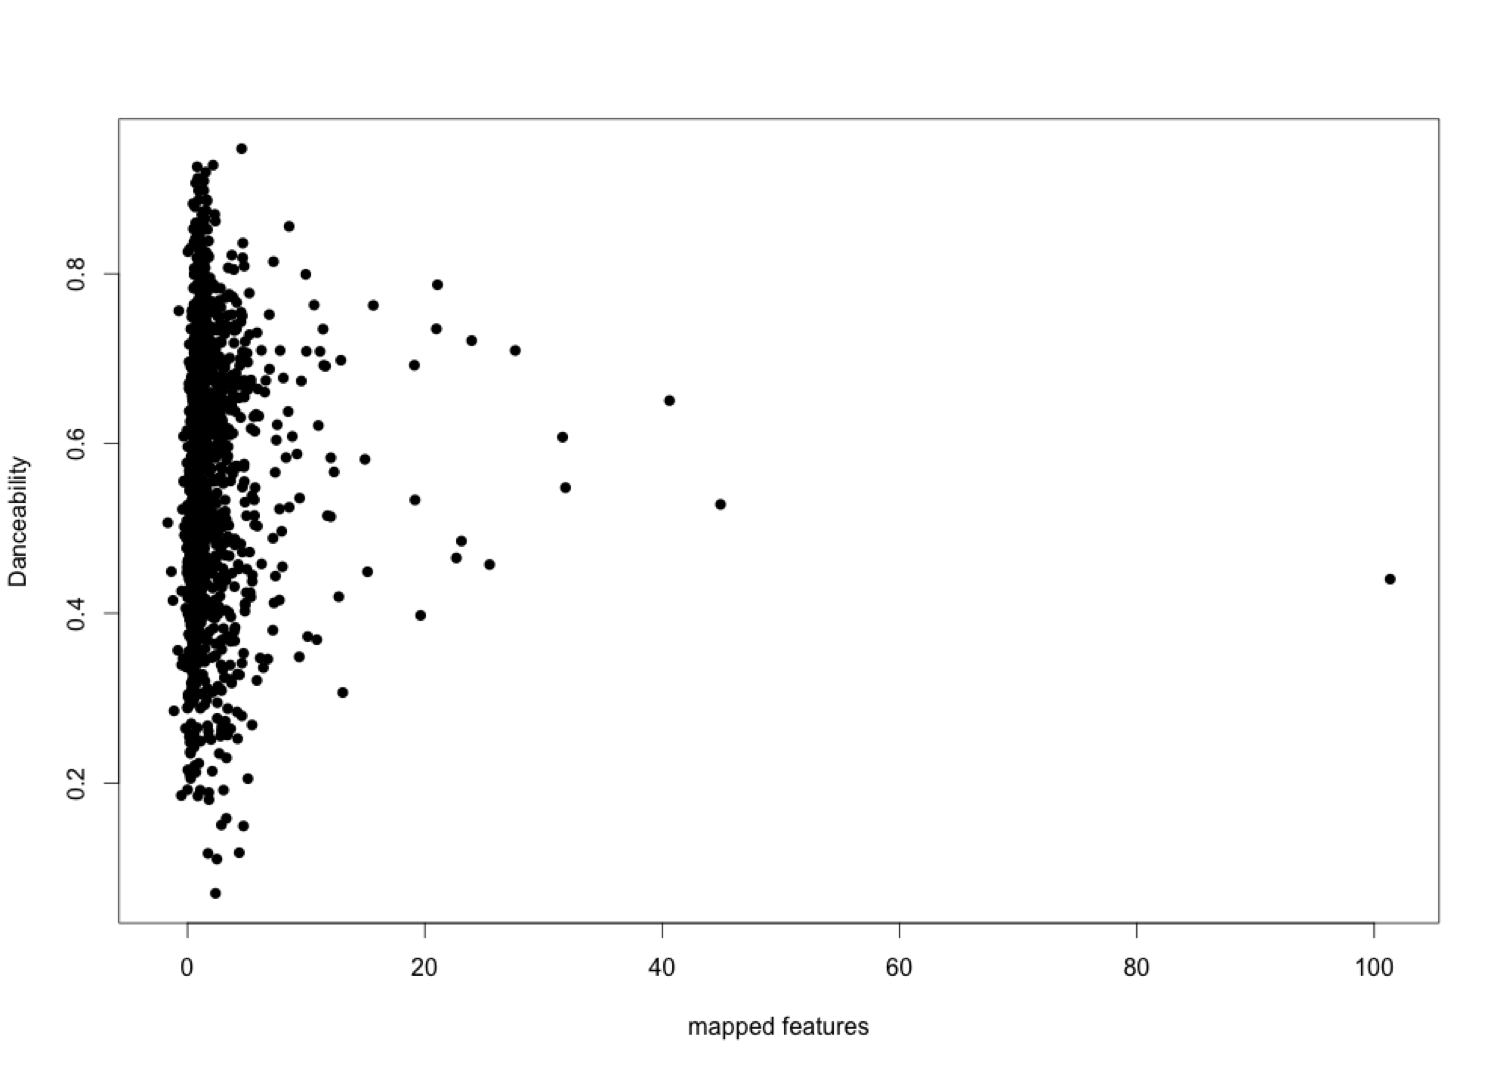
\includegraphics[width=2in]{feature_mapping.png}
\end{center}

We have also started looking into incorporating song lyrics using Bayesian
analysis.  We might use Bayesian analysis to get a float value that
represents ‘lyrical mood’, which we input into our vector in order to
consider how some words suggest a song is more appropriate for dancing
than others. 

\subsection{Problems}
We clearly saw that a lack of data was a major problem in our first
project, and in our current project potential problems still include
dealing with the amount of time it takes to query data from the API and we
are still working through how to include more mathematical analysis such
as computed error bounds, that we need to more concretely plan 

\section{Schedule}
\begin{table}[H]
\label{sample-table}
\vskip 0.1in
\begin{center}
\begin{small}
\begin{tabular}{ll}
\hline
\abovespace\belowspace
Date & Milestone \\
\hline
\abovespace
\textbf{11/11} & \textbf{Progress Report Due}\\
\belowspace
11/13 & Solidify understanding of most relevant features\\
\belowspace
11/15 & Research/training of music similarity functions\\
\belowspace
11/15 & Finish implementation of kNN (Python)\\
\belowspace
11/23 & Finish Testing various feature space mappings\\
\belowspace
11/25 & Fine tune kNN algoirthm (determine $k$)\\
\belowspace
11/28 & Evaluation of Findings\\
\belowspace
12/02 & Finish Poster\\
\belowspace
\textbf{12/04} & \textbf{Poster Presentation}\\
\belowspace
12/12 & Finish Final Report\\
\belowspace
\textbf{12/16} & \textbf{Final Project Report Due}\\
\hline
\end{tabular}
\end{small}
\end{center}
\vskip -0.1in
\end{table}
\end{document} 

% This document was modified from the file originally made available by
% Pat Langley and Andrea Danyluk for ICML-2K. This version was
% created by Lise Getoor and Tobias Scheffer, it was slightly modified  
% from the 2010 version by Thorsten Joachims & Johannes Fuernkranz, 
% slightly modified from the 2009 version by Kiri Wagstaff and 
% Sam Roweis's 2008 version, which is slightly modified from 
% Prasad Tadepalli's 2007 version which is a lightly 
% changed version of the previous year's version by Andrew Moore, 
% which was in turn edited from those of Kristian Kersting and 
% Codrina Lauth. Alex Smola contributed to the algorithmic style files.